% Options for packages loaded elsewhere
\PassOptionsToPackage{unicode}{hyperref}
\PassOptionsToPackage{hyphens}{url}
\PassOptionsToPackage{dvipsnames,svgnames,x11names}{xcolor}
%
\documentclass[
  11pt,
]{article}

\usepackage{amsmath,amssymb}
\usepackage{iftex}
\ifPDFTeX
  \usepackage[T1]{fontenc}
  \usepackage[utf8]{inputenc}
  \usepackage{textcomp} % provide euro and other symbols
\else % if luatex or xetex
  \usepackage{unicode-math}
  \defaultfontfeatures{Scale=MatchLowercase}
  \defaultfontfeatures[\rmfamily]{Ligatures=TeX,Scale=1}
\fi
\usepackage{lmodern}
\ifPDFTeX\else  
    % xetex/luatex font selection
    \setmainfont[]{Aptos}
\fi
% Use upquote if available, for straight quotes in verbatim environments
\IfFileExists{upquote.sty}{\usepackage{upquote}}{}
\IfFileExists{microtype.sty}{% use microtype if available
  \usepackage[]{microtype}
  \UseMicrotypeSet[protrusion]{basicmath} % disable protrusion for tt fonts
}{}
\makeatletter
\@ifundefined{KOMAClassName}{% if non-KOMA class
  \IfFileExists{parskip.sty}{%
    \usepackage{parskip}
  }{% else
    \setlength{\parindent}{0pt}
    \setlength{\parskip}{6pt plus 2pt minus 1pt}}
}{% if KOMA class
  \KOMAoptions{parskip=half}}
\makeatother
\usepackage{xcolor}
\setlength{\emergencystretch}{3em} % prevent overfull lines
\setcounter{secnumdepth}{-\maxdimen} % remove section numbering
% Make \paragraph and \subparagraph free-standing
\makeatletter
\ifx\paragraph\undefined\else
  \let\oldparagraph\paragraph
  \renewcommand{\paragraph}{
    \@ifstar
      \xxxParagraphStar
      \xxxParagraphNoStar
  }
  \newcommand{\xxxParagraphStar}[1]{\oldparagraph*{#1}\mbox{}}
  \newcommand{\xxxParagraphNoStar}[1]{\oldparagraph{#1}\mbox{}}
\fi
\ifx\subparagraph\undefined\else
  \let\oldsubparagraph\subparagraph
  \renewcommand{\subparagraph}{
    \@ifstar
      \xxxSubParagraphStar
      \xxxSubParagraphNoStar
  }
  \newcommand{\xxxSubParagraphStar}[1]{\oldsubparagraph*{#1}\mbox{}}
  \newcommand{\xxxSubParagraphNoStar}[1]{\oldsubparagraph{#1}\mbox{}}
\fi
\makeatother


\providecommand{\tightlist}{%
  \setlength{\itemsep}{0pt}\setlength{\parskip}{0pt}}\usepackage{longtable,booktabs,array}
\usepackage{calc} % for calculating minipage widths
% Correct order of tables after \paragraph or \subparagraph
\usepackage{etoolbox}
\makeatletter
\patchcmd\longtable{\par}{\if@noskipsec\mbox{}\fi\par}{}{}
\makeatother
% Allow footnotes in longtable head/foot
\IfFileExists{footnotehyper.sty}{\usepackage{footnotehyper}}{\usepackage{footnote}}
\makesavenoteenv{longtable}
\usepackage{graphicx}
\makeatletter
\def\maxwidth{\ifdim\Gin@nat@width>\linewidth\linewidth\else\Gin@nat@width\fi}
\def\maxheight{\ifdim\Gin@nat@height>\textheight\textheight\else\Gin@nat@height\fi}
\makeatother
% Scale images if necessary, so that they will not overflow the page
% margins by default, and it is still possible to overwrite the defaults
% using explicit options in \includegraphics[width, height, ...]{}
\setkeys{Gin}{width=\maxwidth,height=\maxheight,keepaspectratio}
% Set default figure placement to htbp
\makeatletter
\def\fps@figure{htbp}
\makeatother

\usepackage{booktabs}
\usepackage{longtable}
\usepackage{array}
\usepackage{multirow}
\usepackage{wrapfig}
\usepackage{float}
\usepackage{colortbl}
\usepackage{pdflscape}
\usepackage{tabu}
\usepackage{threeparttable}
\usepackage{threeparttablex}
\usepackage[normalem]{ulem}
\usepackage{makecell}
\usepackage{xcolor}
\usepackage{pdfpages}
\usepackage{fontspec}
\usepackage[bottom]{footmisc}
\setmainfont{Aptos}[Path="C:/Users/ginow/AppData/Roaming/TinyTeX/texmf-dist/fonts/truetype/aptos/", Extension=".ttf"]
\usepackage{fancyhdr}
\pagestyle{fancy}
\fancyhf{}
\fancyhead[C]{\makebox[\textwidth]{\hspace*{-1cm}
\includegraphics[height=1.9cm]{../Logotipo ENADEL/encabezado_izquierda1.png} \hfill 
\includegraphics[height=1.5cm]{../Logotipo ENADEL/encabezado_derecha.png} \hspace*{-2cm}}}
\fancyfoot[L]{Subsecretaría del Trabajo}
\cfoot{\thepage}
\setlength{\footskip}{10pt}
\setlength{\skip\footins}{15pt}
\setlength{\headheight}{3cm}
\setlength{\headsep}{0.5cm}
\renewcommand{\footrulewidth}{0pt}
\floatplacement{figure}{H}
\floatplacement{table}{H}
\usepackage{geometry}
\geometry{ left=3cm, right=3cm, top=2.5cm, bottom=2.5cm }
\usepackage{placeins}
\usepackage{ragged2e}
\usepackage{float}
\usepackage{setspace}
\renewcommand{\familydefault}{\sfdefault}
\AtBeginDocument{\renewcommand{\baselinestretch}{1.5}\justifying}
\usepackage{xcolor}
\usepackage{pagecolor}
\makeatletter
\@ifpackageloaded{caption}{}{\usepackage{caption}}
\AtBeginDocument{%
\ifdefined\contentsname
  \renewcommand*\contentsname{Tabla de contenidos}
\else
  \newcommand\contentsname{Tabla de contenidos}
\fi
\ifdefined\listfigurename
  \renewcommand*\listfigurename{Listado de Figuras}
\else
  \newcommand\listfigurename{Listado de Figuras}
\fi
\ifdefined\listtablename
  \renewcommand*\listtablename{Listado de Tablas}
\else
  \newcommand\listtablename{Listado de Tablas}
\fi
\ifdefined\figurename
  \renewcommand*\figurename{Figura}
\else
  \newcommand\figurename{Figura}
\fi
\ifdefined\tablename
  \renewcommand*\tablename{Tabla}
\else
  \newcommand\tablename{Tabla}
\fi
}
\@ifpackageloaded{float}{}{\usepackage{float}}
\floatstyle{ruled}
\@ifundefined{c@chapter}{\newfloat{codelisting}{h}{lop}}{\newfloat{codelisting}{h}{lop}[chapter]}
\floatname{codelisting}{Listado}
\newcommand*\listoflistings{\listof{codelisting}{Listado de Listados}}
\makeatother
\makeatletter
\makeatother
\makeatletter
\@ifpackageloaded{caption}{}{\usepackage{caption}}
\@ifpackageloaded{subcaption}{}{\usepackage{subcaption}}
\makeatother

\ifLuaTeX
\usepackage[bidi=basic]{babel}
\else
\usepackage[bidi=default]{babel}
\fi
\babelprovide[main,import]{spanish}
\ifPDFTeX
\else
\babelfont{rm}[]{Aptos}
\fi
% get rid of language-specific shorthands (see #6817):
\let\LanguageShortHands\languageshorthands
\def\languageshorthands#1{}
\ifLuaTeX
  \usepackage{selnolig}  % disable illegal ligatures
\fi
\usepackage{bookmark}

\IfFileExists{xurl.sty}{\usepackage{xurl}}{} % add URL line breaks if available
\urlstyle{same} % disable monospaced font for URLs
\hypersetup{
  pdflang={es},
  colorlinks=true,
  linkcolor={blue},
  filecolor={Maroon},
  citecolor={Blue},
  urlcolor={Blue},
  pdfcreator={LaTeX via pandoc}}


\author{}
\date{}

\begin{document}

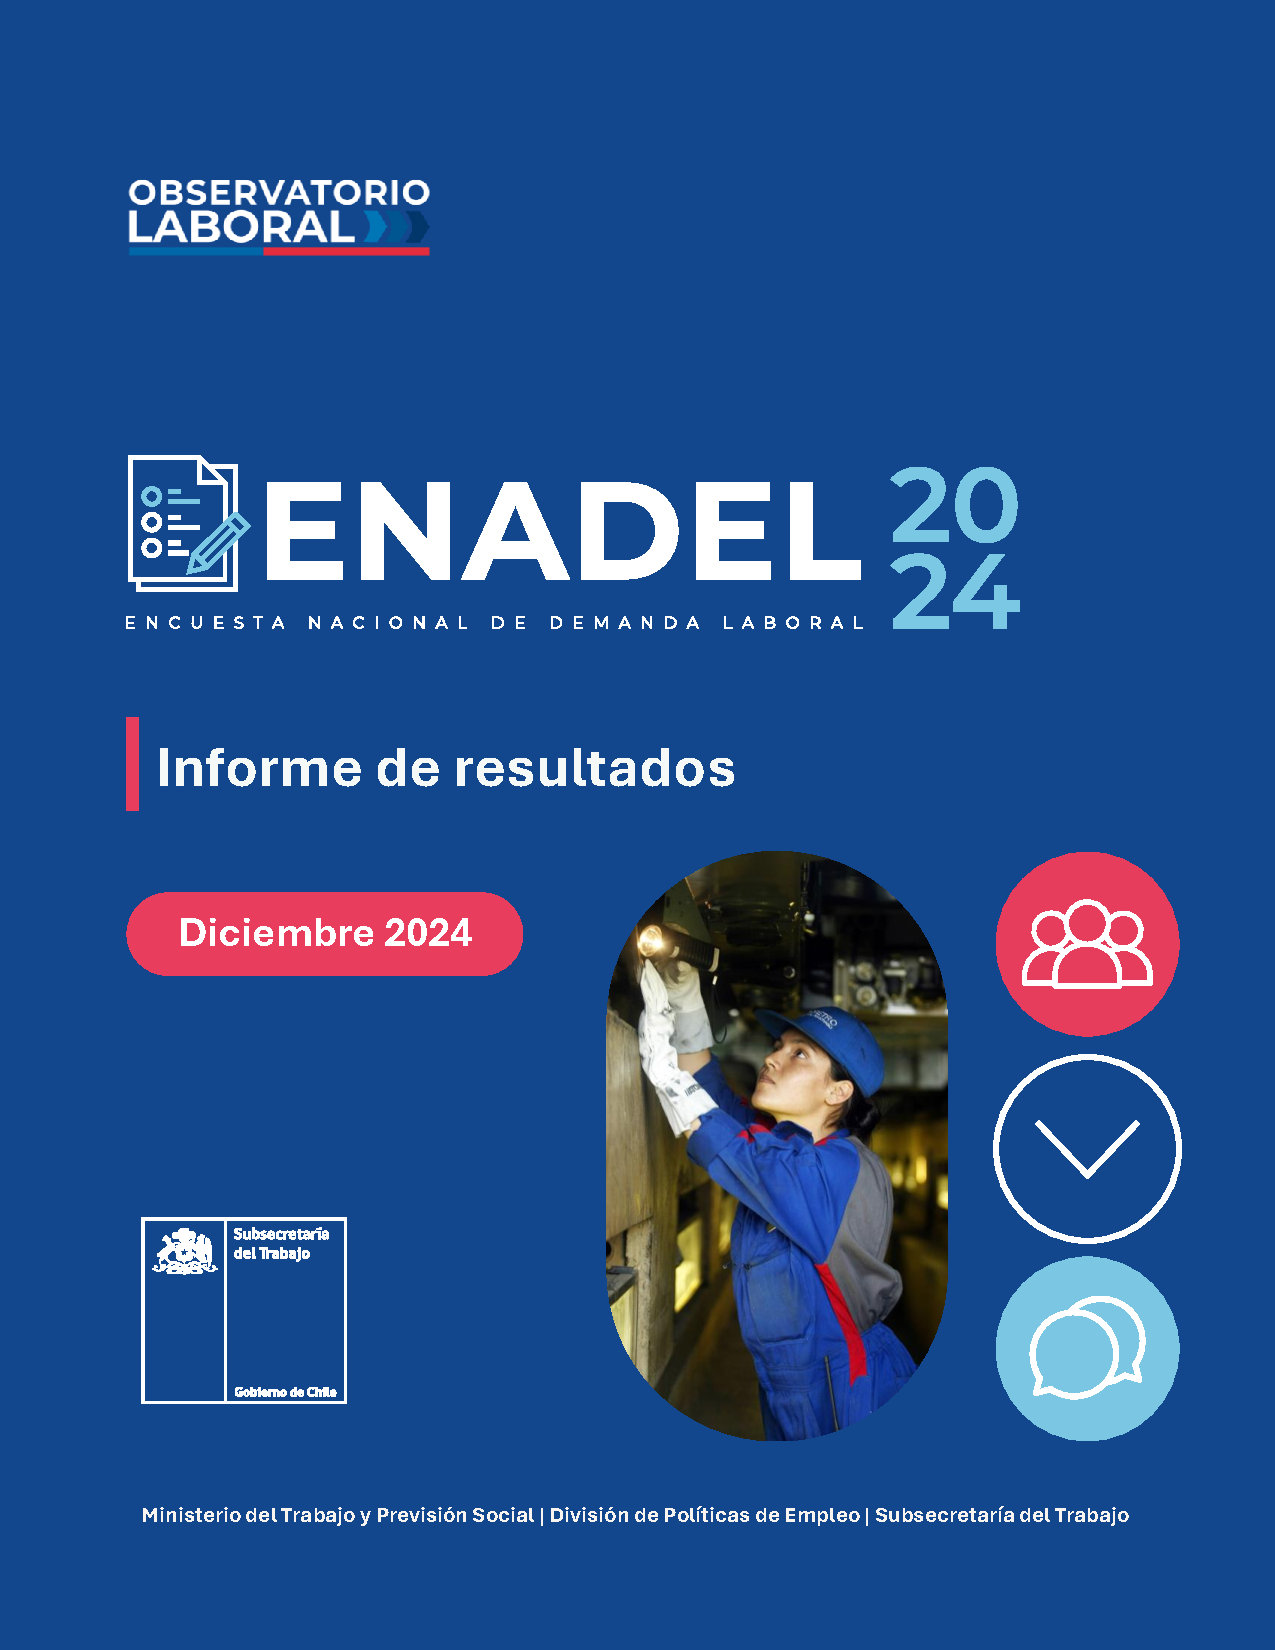
\includepdf[pages=-]{../Quarto/Portada/Portada_ENADEL 2024.pdf}


\definecolor{customblue}{HTML}{12468d}

\pagecolor{customblue} 
\thispagestyle{empty} 
\color{white}

\centering


\includegraphics[width=0.5\textwidth]{../Logotipo ENADEL/Logotipo ENADEL-02.png}
\vspace{2cm}

\noindent Ministerio del Trabajo y Previsión Social

Departamento de intermediación y prospección laboral\textbackslash{}
Subsecretaría del Trabajo

\justifying

El presente documento analiza los resultados de la Encuesta Nacional de
Demanda Laboral (ENADEL) 2024, que busca identificar y caracterizar el
capital humano requerido por las empresas de los distintos sectores
productivos del país, generando información sobre la demanda actual de
ocupaciones de las empresas, detectando requisitos y problemas de
contratación. A diferencia de las versiones anteriores de esta encuesta,
la actual versión abarca 15 sectores de actividad económica, ayuda a
identificar prioridades de capacitación y se añade el foco sobre el
impacto que está teniendo la incorporación de nuevas tecnologías y los
eventos climáticos extremos sobre los trabajadores.

\newpage
\nopagecolor
\color{black}
\renewcommand{\contentsname}{Índice} 
\tableofcontents

\newpage

\subsection{Capítulo I: Contexto y caracterización de
empresas}\label{capuxedtulo-i-contexto-y-caracterizaciuxf3n-de-empresas}

El primer capítulo se centra en contextualizar y caracterizar a las
empresas participantes de la Encuesta Nacional de Demanda Laboral
(ENADEL) 2024. En este apartado se busca comprender la estructura y
distribución de las empresas a nivel nacional, diferenciando por tamaño,
sector productivo y dotación de personal.

Asimismo, se examinan características relevantes de las empresas que
configuran la base del mercado laboral actual, con el fin de establecer
un panorama detallado sobre la composición y dinámica de los sectores
productivos. Este análisis otorga un marco inicial para interpretar la
demanda laboral en los siguientes capítulos, destacando patrones y
diferencias que permiten identificar regiones y sectores de mayor
demanda laboral así como los desafíos futuros asociados a la generación
de empleo en el país.

\FloatBarrier

\subsubsection{Regiones y ubicación de
sucursales}\label{regiones-y-ubicaciuxf3n-de-sucursales}

La muestra de ENADEL 2024 encuesta a 4816 empresas que suman 330937
trabajadores (a nivel muestral). Estas representan a \text{245339}
empresas y \text{17358952} trabajadores a nivel nacional.

La Tabla~\ref{tbl-region} muestra la distribución en las distintas
regiones del país, dónde la Macrozona norte\footnote{La macrozona norte
  corresponde a las regiones de Arica y Parinacota, Tarapacá,
  Antofagasta y Atacama. La macrozona centro incluye las regiones de
  Coquimbo y Valparaíso. La macrozona centro-sur abarca las regiones de
  O'Higgins, Maule, Ñuble y Biobío. La macrozona sur comprende las
  regiones de La Araucanía, Los Ríos y Los Lagos. Finalmente, la
  macrozona austral corresponde a las regiones de Aysén y Magallanes.}
representa un total de \text{14,5}\% de las empresas del país y un
\text{6,8}\% del total de trabajadores. En la Macrozona centro se ubican
el \text{15}\% de las empresas y el \text{14,5}\% de los trabajadores.
Un \text{7,3}\% de las empresas y un \text{6,1}\% de los trabajadores se
encuentran en la región Metropolitana. La Macrozonza Centro Sur
contempla el \text{30,5}\% de las empresas y al \text{29,8}\% de
trabajadores del país. Por su parte, un \text{24,7}\% de las empresas
del país se encuentran en la Macrozona Sur, la que comprende al
\text{40,6}\% de los trabajadores a nivel nacional.

Por último, en la Macrozona Austral se encuentran el \text{7,9}\% de las
empresas y el \text{2,2}\% de los trabajadores de Chile.

\vspace{5mm}

\FloatBarrier

\begin{table}

\caption{\label{tbl-region}Resultados de la encuesta}

\centering{

\centering
\begin{tabular}{>{\raggedright\arraybackslash}p{6cm}>{\raggedright\arraybackslash}p{3cm}>{\raggedright\arraybackslash}p{3cm}}
\toprule
Región & \% Empresas & \% Trabajadores\\
\midrule
Arica y Parinacota & 3,3\% & 1\%\\
Tarapacá & 3,9\% & 1\%\\
Antofagasta & 2,2\% & 0,8\%\\
Atacama & 5,1\% & 4\%\\
Coquimbo & 7,3\% & 9,3\%\\
\addlinespace
Valparaíso & 7,7\% & 5,2\%\\
Metropolitana & 7,3\% & 6,1\%\\
O'Higgins & 9,2\% & 7,8\%\\
Maule & 9,8\% & 7,5\%\\
Ñuble & 9,9\% & 14,3\%\\
\addlinespace
Biobío & 1,6\% & 0,2\%\\
La Araucanía & 2,7\% & 4,6\%\\
Los Ríos & 14,4\% & 32\%\\
Los Lagos & 7,6\% & 4\%\\
Aysén & 3,5\% & 0,8\%\\
\addlinespace
Magallanes & 4,4\% & 1,4\%\\
\bottomrule
\multicolumn{3}{l}{\rule{0pt}{1em}Fuente: Elaboración propia utilizando datos de ENADEL 2024, datos expandidos.}\\
\end{tabular}

}

\end{table}%

\newpage

La Figura~\ref{fig-mapa-sucursal} ilustra las regiones donde las
empresas tienen sucursales, las regiones con más cantidad de sucursales
que corresponden a sedes no principales son Los Ríos, Libertador General
Bernardo O'Higgins y Ñuble con un total de 13110, 8739 y 8236 sucursales
respectivamente. Por su parte, las regiones de Bío-Bío, La Araucanía y
Aisén del General Carlos Ibáñez del Campo registran la menor presencia
de sucursales regionales de las empresas, con 2158 o menos dependencias.

\FloatBarrier

\begin{figure}[H]

\caption{\label{fig-mapa-sucursal}Sucursales por región}

\centering{

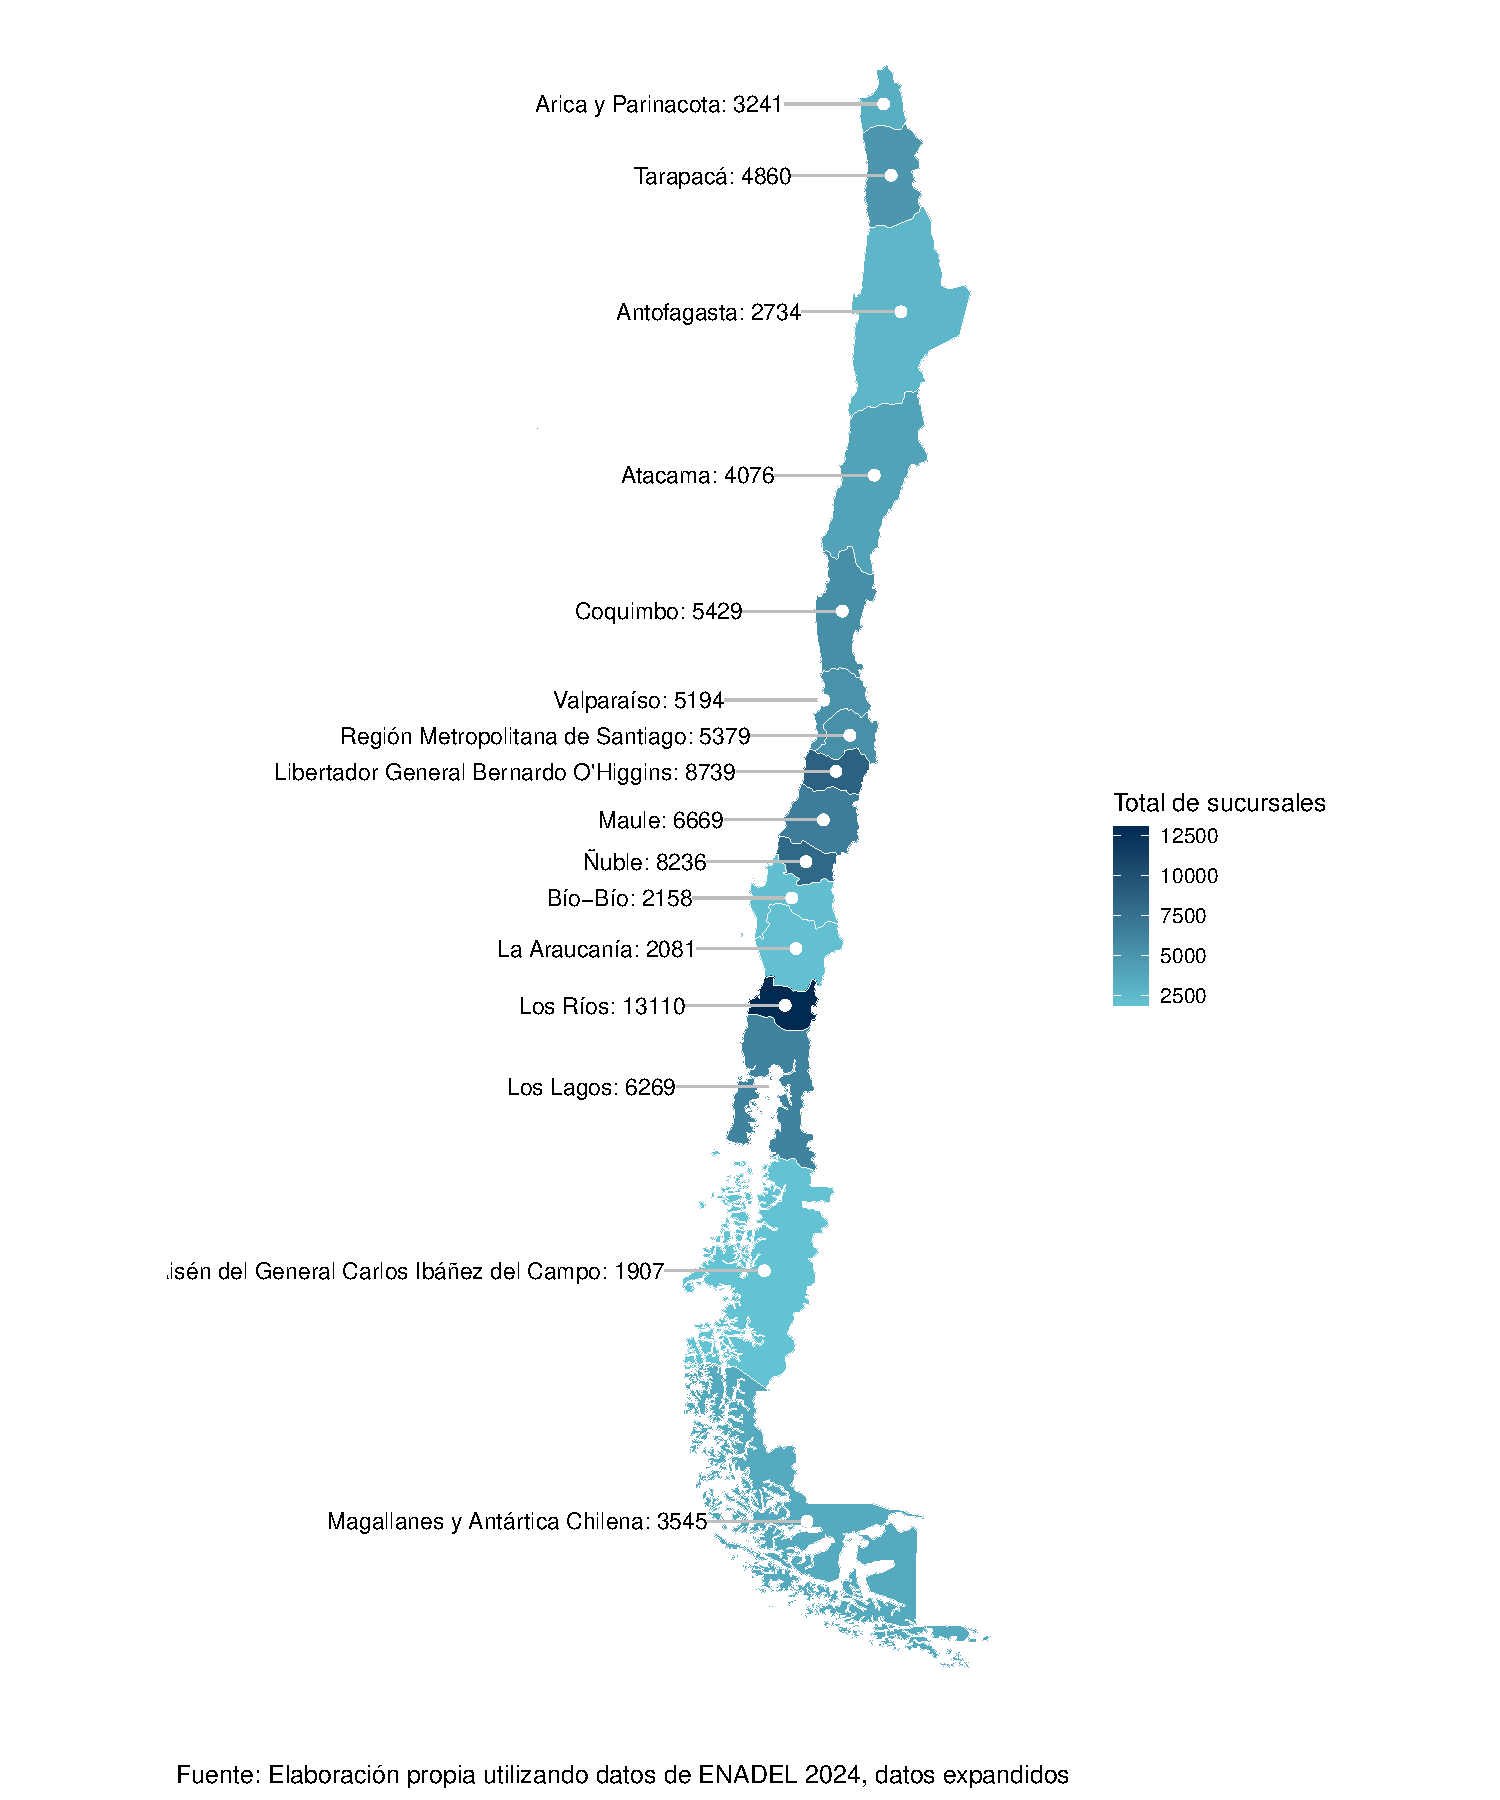
\includegraphics{reporte_2024_files/figure-pdf/fig-mapa-sucursal-1.pdf}

}

\end{figure}%

\FloatBarrier

\subsubsection{Tamaño de empresas (n° de ventas y n° de
trabajadores)}\label{tamauxf1o-de-empresas-n-de-ventas-y-n-de-trabajadores}

La Figura~\ref{fig-combined} muestra como se distribuyen las empresas
por tamaño de empresa, el panel de la izquierda muestra los porcentajes
acorde al tamaño de las empresas según su número de trabajadores. Y en
el panel de la derecha, se aprecia la distribución de las empresas por
tamaño según el volumen de venta de estas.

Con respecto a la primera clasificación, el \text{81,8}\% de las
empresas tiene menos de 50 trabajadores -que representa el \text{20,8}\%
de los trabajadores-. Un \text{12,8}\% de las empresas son medianas de
tamaño (entre 50 y 199 trabajadores), dentro de estas organizaciones se
encuentra el \text{17}\% de los trabajadores del país. Y un \text{5,4}\%
de las empresas corresponde a empresas grandes con 200 trabajadores o
más, lo que equivale al \text{62,2}\% del total de trabajadores.

Si se analiza según tamaño de ventas, un \text{14,5}\% de las empresas
tienen un volumen de venta menores a 2.400 UF (microempresa), el
\text{39,8}\% posee un volumen de venta anual entre 2.400 y 24.999 UF
(``Pequeñas'') y el \text{22}\% venden entre 25.000 y 100.000 UF al año
(``Mediana''). Sin embargo, el \text{49}\% de los trabajadores están en
empresas grandes (más de 100.000 UF).

\FloatBarrier

\begin{figure}[H]

\caption{\label{fig-combined}Gráfico combinado de resultados}

\centering{

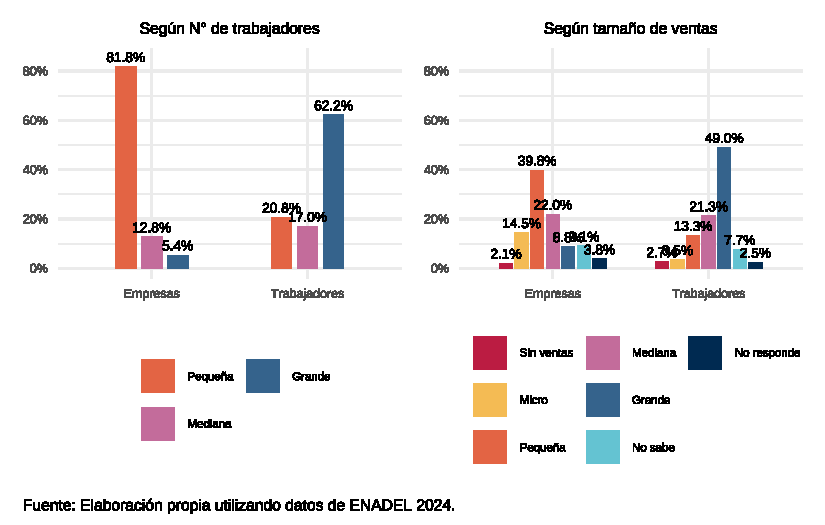
\includegraphics[width=1\textwidth,height=\textheight]{reporte_2024_files/figure-pdf/fig-combined-1.pdf}

}

\end{figure}%

\FloatBarrier

Al revisar la distribución por sector de actividad económica
Tabla~\ref{tbl-acteco} se tiene que el sector de Construcción
(\text{19}\%) , seguido por el sector Transporte y almacenamiento
(\text{14,3}\%) y el sector de Minería (\text{11,1}\%) concentran la
mayor cantidad de empresas a nivel nacional. Con respecto al volumen de
trabajadores, el sector Actividades profesionales y técnicas lidera
(\text{17,7}\%) seguido por el sector Suministro de agua y gestión de
desechos (\text{15,4}\%) y el sector de Agricultura, silvicultura y
pesca que, siendo sector intensivo en trabajo, un \text{9}\% de las
empresas acumula el \text{14,4} de trabajadores y trabajadoras.

\FloatBarrier

\begin{table}

\caption{\label{tbl-acteco}Empresas y trabajadores según sector de
actividad económica}

\centering{

\centering
\begin{tabular}{>{\raggedright\arraybackslash}p{9cm}ll}
\toprule
Actividad Económica & \% Empresas & \% Trabajadores\\
\midrule
Actividades profesionales y técnicas & 8,3\% & 17,7\%\\
Suministro de agua y gestión de  desechos & 9,9\% & 15,4\%\\
Agricultura, silvicultura y pesca & 9\% & 14,4\%\\
Construcción & 19\% & 14,2\%\\
Minería & 11,1\% & 11,4\%\\
\addlinespace
Comercio & 9,4\% & 8,6\%\\
Transporte y almacenamiento & 14,3\% & 5\%\\
Actividades inmobiliarias & 4,9\% & 3,6\%\\
Suministro de electricidad y gas & 2,3\% & 2,8\%\\
Servicios administrativos y de apoyo & 2,8\% & 2,1\%\\
\addlinespace
Alojamiento y de servicio de comida & 3,6\% & 1,8\%\\
Actividades financieras y de seguros & 3,2\% & 1,7\%\\
Industrias manufactureras & 1,1\% & 0,7\%\\
Información y comunicaciones & 1,2\% & 0,7\%\\
\bottomrule
\multicolumn{3}{l}{\rule{0pt}{1em}Fuente: Elaboración propia utilizando datos de ENADEL 2024, datos expandidos.}\\
\end{tabular}

}

\end{table}%

\FloatBarrier

\subsubsection{Estructura corporativa}\label{estructura-corporativa}

En este subapartado se analiza la distribución de las empresas a nivel
nacional según sus características de estructura corporativa. En primer
lugar, se examina el tipo de propiedad de las empresas, diferenciando
entre privadas (nacionales o extranjeras), estatales y mixtas.
Posteriormente, se estudia la distribución de las empresas que prestan
servicios bajo la figura de subcontratación, considerando tanto el
sector de actividad económica como la región. Finalmente, se describe la
distribución de las organizaciones según su pertenencia a conglomerados
y gremios empresariales.

La Tabla~\ref{tbl-tipo_propiedad} muestra la distribución de las
empresas según su tipo de propiedad. Se presentan los datos en términos
de tamaño muestral de empresas, cantidad de empresas expandidas a nivel
poblacional, número de trabajadores en la muestra y trabajadores
representados a nivel poblacional. La gran mayoría de las organizaciones
corresponden al tipo de propiedad Privada nacional, que representa el
\text{97}\% de las empresas y concentra el \text{85,1}\% de los
trabajadores del país. En contraste, otros tipos de propiedad tienen una
representación significativamente menor. Por ejemplo, sólo el
\text{1,7}\% corresponde a empresas del tipo de propiedad Privada
extranjera, lo que equivale a un total del \text{9,7}\% de los
trabajadores del país. A su vez, el \text{0,4}\% corresponde a empresas
del tipo de propiedad Estatal, lo que equivale al \text{2,1}\% de los
trabajadores. Y un \text{0,9}\% corresponde a empresas del tipo de
propiedad Mixta, conteniendo el \text{9,7}\% de los trabajadores del
país.

\begin{table}

\caption{\label{tbl-tipo_propiedad}Tipo de propiedad de empresas}

\centering{

\centering
\begin{tabular}{>{\raggedright\arraybackslash}p{3cm}>{\raggedleft\arraybackslash}p{2.5cm}>{\raggedleft\arraybackslash}p{2.5cm}>{\raggedleft\arraybackslash}p{2.5cm}>{\raggedleft\arraybackslash}p{2.5cm}}
\toprule
Tipo de propiedad & Empresas (Muestra) & Empresas Estimadas & Trabajadores (Muestra) & Trabajadores Estimados\\
\midrule
Privada nacional & 4677 & 238074 & 277885 & 14776364\\
Privada extranjera & 78 & 4064 & 36729 & 1682395\\
Estatal & 21 & 1005 & 6528 & 357124\\
Mixta & 40 & 2195 & 9795 & 543070\\
Total & 4816 & 245338 & 330937 & 17358953\\
\bottomrule
\multicolumn{5}{l}{\rule{0pt}{1em}Fuente: Elaboración propia utilizando datos de ENADEL 2024, datos expandidos.}\\
\end{tabular}

}

\end{table}%

En la Figura~\ref{fig-subcontratos_sector} se aprecia la distribución de
empresas que prestan servicios a otras empresas a través del
subcontrato\footnote{La subcontratación se entiende como el trabajo
  realizado para un empleador denominado contratista o subcontratista,
  quien ejecuta obras o servicios por cuenta y riesgo propio para una
  empresa principal, dueña de la obra o faena.} según sector de
actividad económica. Los sectores de actividad económica con mayor
presencia de empresas que prestan servicios de subcontrato son los
sectores de Construcción (\text{17,9}\%), Transporte y almacenamiento
(\text{16,7}\%) y Servicios administrativos y de apoyo (\text{13,4}\%)
respectivamente. Los sectores que tienen menor presencia de empresas que
prestan servicios de subcontratación son los sectores de Actividades
inmobiliarias (\text{1,3}\%), Suministro de electricidad y gas
(\text{1,1}\%) y Actividades financieras y de seguros (\text{0,6}\%).

\begin{figure}[H]

\caption{\label{fig-subcontratos_sector}Gráfico subcontrato según sector
de actividad económica}

\centering{

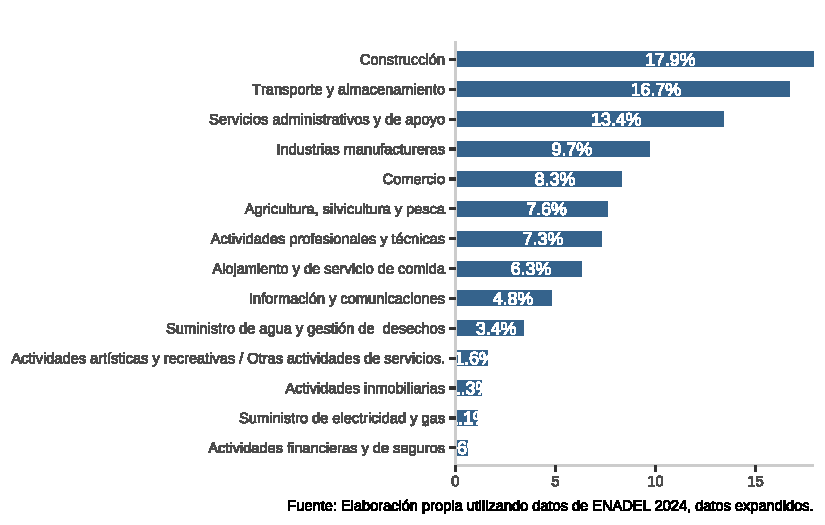
\includegraphics[width=1\textwidth,height=\textheight]{reporte_2024_files/figure-pdf/fig-subcontratos_sector-1.pdf}

}

\end{figure}%

La Tabla~\ref{tbl-subcontratos_region} indica la distribución de las
empresas que prestan servicios bajo la figura del subcontrato según
región de ubicación de la empresa, la región de Biobío es la que posee
la mayor parte (\text{14,2}\%) de empresas subcontratistas del país.
Seguida por la región, del Los Lagos la que concentra el \text{9}\% de
empresas subcontratistas. En tercer lugar, la región de La Araucanía
posee el \text{8,7}\% de este tipo de relación contractual.

\begin{table}

\caption{\label{tbl-subcontratos_region}Distribución regional de
Empresas que Operan mediante Subcontratación}

\centering{

\centering
\begin{tabular}{ll}
\toprule
Región & \% Empresas en subcontrato\\
\midrule
Arica y Parinacota & 3,6\%\\
Tarapacá & 3,4\%\\
Antofagasta & 5,2\%\\
Atacama & 5,2\%\\
Coquimbo & 4,7\%\\
\addlinespace
Valparaíso & 6,7\%\\
Metropolitana & 6,7\%\\
O'Higgins & 5,4\%\\
Maule & 8,1\%\\
Ñuble & 7,2\%\\
\addlinespace
Biobío & 14,2\%\\
La Araucanía & 8,7\%\\
Los Ríos & 7\%\\
Los Lagos & 9\%\\
Aysén & 2,3\%\\
\addlinespace
Magallanes & 2,9\%\\
\bottomrule
\multicolumn{2}{l}{\rule{0pt}{1em}Fuente: Elaboración propia utilizando datos de ENADEL 2024, datos expandidos.}\\
\end{tabular}

}

\end{table}%

La Tabla~\ref{tbl-conglomerado_gremio} presenta los porcentajes de las
empresas que pertencen a conglomerados y gremios\footnote{Un
  conglomerado es un grupo de empresas dedicadas a negocios no
  necesariamente relacionados, pero que tienen un controlador o
  accionista mayoritario común o que se encuentra relacionado mediante
  pactos o sociedades. Estos conglomerados ejercen control sobre las
  empresas afiliadas mediante estructuras piramidales, series
  accionarias preferentes y tenencias cruzadas de acciones (La Porta et
  al., 1999; Wolfenzon, 1999; Bebchuck, Kraakman y Triantis, 1999). En
  Chile, según el Decreto Ley 2757, los gremios empresariales
  corresponden a un tipo de asociación voluntaria de empresas que
  pertenecen a un mismo sector económico o industria, con el propósito
  de representar y defender intereses comunes}. Se aprecia que los
sectores de Comercio con Transporte y almacenamiento y Agricultura,
silvicultura y pesca poseen los mayores niveles de empresas
conglomeradas con el \text{14,7}\%, \text{11,7}\% y \text{11,6}\% de
empresas correspondientes.

Con respecto al poder asociativo de las empresas, el \text{15,6}\% de
las empresas del sector Comercio pertenecen a un gremio empresarial. De
igual forma, el sector Alojamiento y de servicio de comida presenta un
\text{15,6}\% de empresas asociadas, mientras que el sector
\text{15,6}\% cuenta con un Construcción de empresas pertenecientes a
algún gremio empresarial.

\FloatBarrier

\begin{table}

\caption{\label{tbl-conglomerado_gremio}Empresas pertenecientes a
Conglomerados y Gremios}

\centering{

\centering
\begin{tabular}{>{\raggedright\arraybackslash}p{11cm}ll}
\toprule
Actividad Económica & \% Conglomerados & \% Gremios\\
\midrule
Comercio & 14,7\% & 15,6\%\\
Transporte y almacenamiento & 11,7\% & 10\%\\
Agricultura, silvicultura y pesca & 11,6\% & 10,1\%\\
Industrias manufactureras & 11,2\% & 11\%\\
Construcción & 10,7\% & 14,5\%\\
\addlinespace
Servicios administrativos y de apoyo & 9,5\% & 4,6\%\\
Alojamiento y de servicio de comida & 6,8\% & 15,6\%\\
Actividades inmobiliarias & 5,5\% & 3,9\%\\
Actividades profesionales y técnicas & 3,7\% & 4,2\%\\
Actividades artísticas y recreativas / Otras actividades de servicios. & 3,7\% & 1,7\%\\
\addlinespace
Actividades financieras y de seguros & 3,7\% & 1,4\%\\
Información y comunicaciones & 3,3\% & 4,5\%\\
Suministro de agua y gestión de  desechos & 2\% & 1,8\%\\
Suministro de electricidad y gas & 1,8\% & 1\%\\
\bottomrule
\multicolumn{3}{l}{\rule{0pt}{1em}Fuente: Elaboración propia utilizando datos de ENADEL 2024, datos expandidos.}\\
\end{tabular}

}

\end{table}%

\FloatBarrier

\newpage

\subsection{Capítulo II: Demanda Laboral y Ocupaciones de Difícil
Cobertura}\label{capuxedtulo-ii-demanda-laboral-y-ocupaciones-de-difuxedcil-cobertura}

A continuación, se identifica y caracteriza la demanda laboral de las
empresas durante 2024. En primer lugar, se presentan las cifras
relativas a la dotación actual de personal en las empresas, seguido de
un análisis de las salidas y contrataciones realizadas para determinar
la demanda de trabajo de las organizaciones, incluyendo los principales
perfiles ocupacionales contratados, sus competencias y los requisitos
asociados.En segundo lugar, se presentan las vacantes
actuales\footnote{Número de ofertas de trabajo que se esperan abrir en
  lo que queda del año 2024.} y futuras\footnote{Número de ofertas de
  trabajo que se esperan abrir durante el año 2025.}. Para finalizar el
análisis se identifican las principales ocupaciones de difícil cobertura
presentando las dificultades más relevantes que enfrentan estas
posiciones no cubiertas.

\subsubsection{Dotación}\label{dotaciuxf3n}

En cuanto a la dotación actual de las empresas, la
Tabla~\ref{tbl-dotacion_resumen} indica que la cantidad actual de
personas empleadas asciende a un total de 17358952 a nivel nacional.
Además, se aprecia que la mayor parte de la dotación de trabajadores se
encuentra en la categoría de Contrato Indefinido con un total de
11776473 trabajadores, de los cuales el 32,7\% corresponden a mujeres y
un 67,2\% a personal masculino. Si bien la distribución según sexo del
trabajador se mantiene en el resto de categorías contractuales, es la
categoría de Honorario donde hay mayor presencia de mujeres
trabajadoras, lo que da cuenta de que las mujeres se encuentran en una
condición de independencia y flexibilidad, pero al mismo tiempo de mayor
inestabilidad y ausencia de protección laboral.

\FloatBarrier

\begin{table}

\caption{\label{tbl-dotacion_resumen}Dotación actual de las empresas
segpun tipo de relación contractual}

\centering{

\centering
\begin{tabular}{>{\raggedright\arraybackslash}p{3cm}rrrll}
\toprule
Categoría & Total & Mujer & Hombre & \% Mujer & \% Hombre\\
\midrule
Indefinido & 11776473 & 3852312 & 7915540 & 32,7\% & 67,2\%\\
Plazo fijo & 5056494 & 1656658 & 3399548 & 32,8\% & 67,2\%\\
Honorario & 302955 & 137111 & 165803 & 45,3\% & 54,7\%\\
Dotación total & 17358952 & 5713742 & 11645210 & 32,9\% & 67,1\%\\
\bottomrule
\multicolumn{6}{l}{\rule{0pt}{1em}Fuente: Elaboración propia utilizando datos de ENADEL 2024, datos expandidos.}\\
\end{tabular}

}

\end{table}%

\FloatBarrier

\subsubsection{Vacantes y Salidas}\label{vacantes-y-salidas}

La Figura~\ref{fig-vacantes} presenta las vacantes actuales\footnote{Número
  de ofertas de trabajo o vacantes abiertas al 31 de mayo del 2024.} y
las vacantes futuras, que corresponden a la cantidad estimada de puestos
de trabajo que se abrirán en los próximos doce meses. Actualmente,
existen 964882 vacantes disponibles. En cuanto a las vacantes futuras,
estas se dividen en dos categorías: los puestos de trabajo previstos
para el resto del año 2024 (3235711) y las ofertas de empleo proyectadas
para el año 2025 (4620639).

\FloatBarrier

\begin{figure}[H]

\caption{\label{fig-vacantes}Gráfico Vacantes}

\centering{

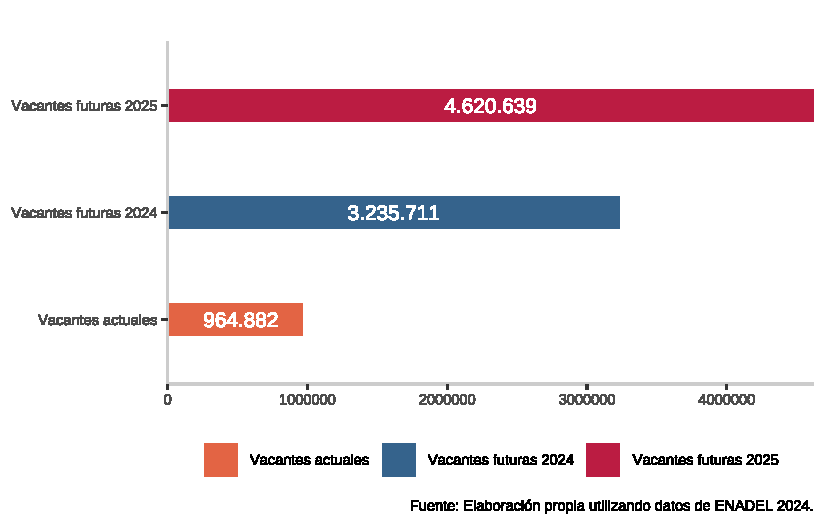
\includegraphics[width=1\textwidth,height=\textheight]{reporte_2024_files/figure-pdf/fig-vacantes-1.pdf}

}

\end{figure}%

En la Figura~\ref{fig-salidas_contrataciones} aparecen los porcentajes
correspondientes a las salidas (renuncias, despidos o ceses)\footnote{Renuncias
  y Ceses, terminaciones de empleados/as permanentes, de corto plazo o
  estacionales.} y contrataciones diferenciando por sexo de los
trabajadores. Durante los últimos 12 meses a nivel nacional hubo un
total de \text{1569395} renuncias, de las cuales el \text{34,7}\%
corresponde a renuncias hechas por mujeres, mientras que el
\text{64,5}\% de estas corresponden a renuncias hechas por hombres.

En cuanto a despidos (y ceses) \footnote{Ceses, terminaciones de
  empleados/as permanentes, de corto plazo o estacionales.}, en el
gráfico se observa que a nivel nacional existió un total de
\text{7040137}, de los cuales el \text{34,8}\% corresponde a casos de
despidos o terminaciones de empleos ocupados por mujeres, y un
\text{64,4}\% corresponde a despidos o ceses cuyos puestos de trabajos
eran ocupados por hombres.

\FloatBarrier

\begin{figure}[H]

\caption{\label{fig-salidas_contrataciones}Gráfico salidas y
contrataciones}

\centering{

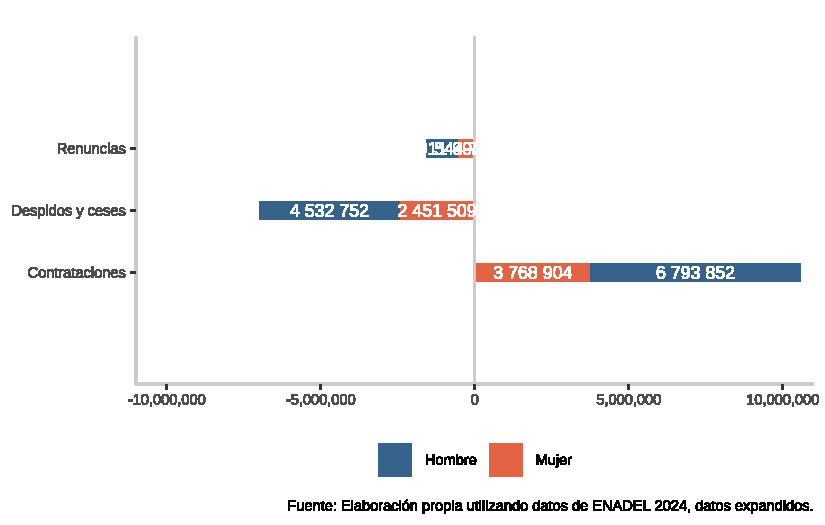
\includegraphics[width=1\textwidth,height=\textheight]{reporte_2024_files/figure-pdf/fig-salidas_contrataciones-1.pdf}

}

\end{figure}%

\subsubsection{Contrataciones últimos 12
meses}\label{contrataciones-uxfaltimos-12-meses}

La Tabla~\ref{tbl-contratados_u12} sólo muestra aquellas ocupaciones
para las cuáles el coeficiente de variación es menor a 50\%\footnote{La
  convención es considerar cómo robustas estimaciones con un cv menor al
  15\%. Dado que estas son pocas, se presentan todas las ocupaciones con
  un cv menor a 50\%.}. Las ocupaciones más contratadas en los últimos
12 meses fueron ``Auxiliares de aseo de oficinas, hoteles y otros
establecimientos'' con 222241 contrataciones, en segundo lugar con
171388 contrataciones, ``Obreros de explotaciones agrícolas'' y
``Empleados encargados del control de abastecimiento e inventario'' con
141683 contrataciones. \FloatBarrier

\begin{table}

\caption{\label{tbl-contratados_u12}Contratados últimos 12 meses, por
ocupación.}

\centering{

\centering
\begin{tabular}{r>{\raggedright\arraybackslash}p{10cm}rl}
\toprule
CIUO\_08 & Glosa & Contratados & cv\\
\midrule
9112 & Auxiliares de aseo de oficinas, hoteles y otros establecimientos & 222241 & 31,4\%\\
9211 & Obreros de explotaciones agrícolas & 171388 & 36,6\%\\
4321 & Empleados encargados del control de abastecimiento e inventario & 141683 & 34,3\%\\
5414 & Guardias de seguridad & 124867 & 48,5\%\\
3123 & Supervisores de la construcción & 86389 & 29,9\%\\
\addlinespace
3113 & Técnicos en electricidad & 85976 & 37\%\\
2142 & Ingenieros civiles, ingenieros en construcción y constructores civiles & 79051 & 34,3\%\\
9313 & Obreros de la construcción de edificios & 70138 & 36,8\%\\
4110 & Trabajadores de tareas administrativas generales & 54087 & 49,2\%\\
9412 & Ayudantes de cocina & 51284 & 32,1\%\\
\addlinespace
7112 & Albañiles & 46799 & 45\%\\
\bottomrule
\multicolumn{4}{l}{\rule{0pt}{1em}Fuente: Elaboración propia utilizando datos de ENADEL 2024, datos expandidos.}\\
\end{tabular}

}

\end{table}%

\FloatBarrier

La Tabla~\ref{tbl-contratados_sector} muestra la comparativa entre los
sectores de actividad económica con respecto a la cantidad de puestos de
trabajos contratados los últimos 12 meses, el sector de Agricultura,
silvicultura y pesca con 3047175 contrataciones. En segundo lugar, el
sector de Servicios administrativos y de apoyo contrató un total de
1197570 personas, seguido del sector de Construcción con un total de
498805 ocupaciones contratadas durante los últimos 12 meses. Dentro de
los sectores que menos vacantes contratados tuvieron fueron los sectores
de Actividades inmobiliarias con 27375 puestos de trabajo, el sector
Actividades financieras y de seguros con 16032 vacantes contratadas y el
sector Suministro de electricidad y gas con 10017 vacantes contratadas
durante el último año.

\FloatBarrier

\begin{table}

\caption{\label{tbl-contratados_sector}Contratados últimos 12 meses por
sector de actividad económica.}

\centering{

\centering
\begin{tabular}{>{\raggedright\arraybackslash}p{9cm}r}
\toprule
Glosa & Contratados\\
\midrule
Agricultura, silvicultura y pesca & 3047175\\
Servicios administrativos y de apoyo & 1197570\\
Construcción & 498805\\
Industrias manufactureras & 449081\\
Comercio & 356693\\
\addlinespace
Transporte y almacenamiento & 253568\\
Alojamiento y de servicio de comida & 118735\\
Actividades profesionales y técnicas & 86084\\
Suministro de agua y gestión de  desechos & 44339\\
Actividades artísticas y recreativas / Otras actividades de servicios. & 37359\\
\addlinespace
Información y comunicaciones & 27481\\
Actividades inmobiliarias & 27375\\
Actividades financieras y de seguros & 16032\\
Suministro de electricidad y gas & 10017\\
\bottomrule
\multicolumn{2}{l}{\rule{0pt}{1em}Fuente: Elaboración propia utilizando datos de ENADEL 2024, datos expandidos.}\\
\end{tabular}

}

\end{table}%

\subsubsection{Ocupaciones de Difícil
Cobertura}\label{ocupaciones-de-difuxedcil-cobertura}

Las ocupaciones de difícil cobertura son aquellas ocupaciones o puestos
de trabajo que los empleadores encuentran difíciles de cubrirpor
diferentes causas como la escasez de trabajadores con las competencias,
habilidades o experiencia necesarias. Estas dificultades pueden
originarse por la falta de oferta de mano de obra calificada, brechas de
habilidades técnicas o blandas, condiciones laborales poco atractivas
(como salarios bajos o jornadas extensas), o problemas de localización
geográfica que limitan el acceso a trabajadores en regiones específicas.
Identificar estas ocupaciones permite entender las dinámicas del mercado
laboral y los desafíos que enfrentan distintos sectores productivos del
país.

Medir este tipo de ocupaciones es fundamental porque facilita el
emparejamiento (\textbf{match}) entre la oferta y la demanda laboral,
orientando programas de capacitación y formación hacia las necesidades
reales del mercado. Además, ayuda a optimizar los procesos de
intermediación laboral y permite anticipar tendencias, ayudando a
trabajadores y estudiantes a tomar decisiones informadas sobre su
desarrollo profesional. Al mismo tiempo, contribuye a reducir
desigualdades regionales al focalizar esfuerzos en zonas rezagadas,
fortaleciendo el capital humano y mejorando la competitividad del país.
En síntesis, esta medición es clave para implementar políticas públicas
más efectivas y promover una fuerza laboral adaptada a los desafíos
económicos actuales y futuros.

La Tabla~\ref{tbl-cuadro8_odc} sólo muestra aquellas para las cuáles el
coeficiente de variación es menor a 40\%\footnote{La convención es
  considerar cómo robustas estimaciones con un cv menor al 15\%. Dado
  que esto no se cumple, se presentan todas las ocupaciones con un cv
  menor a 40\%.}. La ocupación más dificiles de cubrir es la de Obreros
de explotaciones agrícolas con un total de 1827 vacantes sin llenar. En
segundo lugar, la ocupación Obreros de la construcción de edificios tuvo
un total de 1438 vacantes sin llenar. La ocupación de Guardias de
seguridad tuvo un total de 1117 vacantes sin cubrir.

\begin{table}

\caption{\label{tbl-cuadro8_odc}Ocupaciones de difícil cobertura, ENADEL
2024.}

\centering{

\centering
\begin{tabular}{r>{\raggedright\arraybackslash}p{9cm}rl}
\toprule
CIUO 08 & Glosa & Vacantes & CV\\
\midrule
9211 & Obreros de explotaciones agrícolas & 1827 & 25,5\%\\
9313 & Obreros de la construcción de edificios & 1438 & 39,8\%\\
5414 & Guardias de seguridad & 1117 & 29,6\%\\
5230 & Vendedores de entradas (entretenciones y eventos deportivos) y cajeros de comercio & 1044 & 28,9\%\\
9412 & Ayudantes de cocina & 915 & 30,6\%\\
\addlinespace
5131 & Garzones de mesa & 849 & 29,1\%\\
5223 & Vendedores y asistentes de venta de tiendas, almacenes y puestos de mercado & 684 & 34,2\%\\
4110 & Trabajadores de tareas administrativas generales & 553 & 38,6\%\\
7233 & Mecánicos y reparadores de máquinas agrícolas e industriales & 513 & 36,9\%\\
3123 & Supervisores de la construcción & 512 & 37,5\%\\
\addlinespace
7212 & Soldadores y oxicortadores & 480 & 32,6\%\\
4321 & Empleados encargados del control de abastecimiento e inventario & 444 & 39,1\%\\
5245 & Bomberos de gasolineras & -3637 & -101,9\%\\
8332 & Conductores de camiones pesados y de alto tonelaje & -7785 & -108,4\%\\
8342 & Operadores de máquinas de movimiento de tierras & -8066 & -102,4\%\\
\bottomrule
\multicolumn{4}{l}{\rule{0pt}{1em}Fuente: Elaboración propia utilizando datos de ENADEL 2024, datos expandidos.}\\
\end{tabular}

}

\end{table}%

\subsubsection{Principales Dificultades}\label{principales-dificultades}

La Tabla~\ref{tbl-dificultad} muestra las principales dificultades de
contratación. La dificultad más reportada es la de ``Candidatos sin
competencias o habilidades técnicas requeridas'', presente en el
\text{26}\% de los casos, seguida por ``Falta de postulantes'' con un
\text{23,4}\% y ``Condiciones laborales (ubicación, horario y/o jornada)
no aceptadas'', que representa el \text{10}\% del total de los
principales cargos con dificultades de contratación.

\begin{table}

\caption{\label{tbl-dificultad}Dificultades de contratación.}

\centering{

\centering
\begin{tabular}{>{\raggedright\arraybackslash}p{10cm}>{\raggedright\arraybackslash}p{3cm}>{\raggedright\arraybackslash}p{3cm}}
\toprule
Primera dificultad & \% de 1ra dificultad & \% del total\\
\midrule
Candidatos sin competencias o habilidades técnicas requeridas & 24,7\% & 26\%\\
Falta de postulantes & 23,7\% & 23,4\%\\
Condiciones laborales (ubicación, horario y/o jornada) no aceptadas & 10\% & 10\%\\
Otra dificultad & 9\% & 9,5\%\\
Candidatos sin la experiencia mínima requerida & 9,5\% & 8,6\%\\
\addlinespace
Renumeración ofrecida no aceptada & 8,8\% & 8,3\%\\
Candidatos sin habilidades blandas o socioemocionales requeridas & 7,1\% & 7,1\%\\
Candidatos sin licencias, certificaciones o requisitos legales & 5,6\% & 5,3\%\\
Candidatos sin nivel educacional requerido & 1,7\% & 1,8\%\\
\bottomrule
\multicolumn{3}{l}{\rule{0pt}{1em}Fuente: Elaboración propia utilizando datos de ENADEL 2024, datos expandidos.}\\
\end{tabular}

}

\end{table}%

\newpage

\subsection{Capítulo III: Capacitación y
Habilidades}\label{capuxedtulo-iii-capacitaciuxf3n-y-habilidades}

\subsubsection{Organismo Técnico Intermedio para
capacitación}\label{organismo-tuxe9cnico-intermedio-para-capacitaciuxf3n}

\subsubsection{Capacitaciones de la
empresa}\label{capacitaciones-de-la-empresa}

\subsubsection{Competencias en que se
capacita}\label{competencias-en-que-se-capacita}

\subsubsection{Fuentes de financiamiento de la
capacitación}\label{fuentes-de-financiamiento-de-la-capacitaciuxf3n}

\subsection{Capítulo IV:
Transiciones}\label{capuxedtulo-iv-transiciones}

\subsubsection{Eventos climáticos
extremos}\label{eventos-climuxe1ticos-extremos}

\subsubsection{Medidas de Cuidado del
medioambiente}\label{medidas-de-cuidado-del-medioambiente}

\subsubsection{Digitalización y
Automatización}\label{digitalizaciuxf3n-y-automatizaciuxf3n}

\paragraph{Cambios en dotación de
personal}\label{cambios-en-dotaciuxf3n-de-personal}

\paragraph{Creación de nuevos puestos de
trabajo}\label{creaciuxf3n-de-nuevos-puestos-de-trabajo}

\paragraph{Dificultad para llenar
vacantes}\label{dificultad-para-llenar-vacantes}




\end{document}
